\chapter{資料集介紹與特徵設計}
{本章總共分成三個部分,首先第一節將介紹原始資料(raw data)之詳細組成資訊,原始資料包含:網頁瀏覽歷史紀錄、使用者之詳細個人資訊以及大六性格特質測驗分數。第二節介紹資料前處理之過程與想法。第三節則說明特徵選擇之原因。}

\section{資料集中各類資訊介紹}
\subsection{資料集中網頁瀏覽歷史紀錄之介紹}
{
本篇論文所使用之資料集是取自 $672$ 位使用者之 Google Chrome 網頁瀏覽器之網頁瀏覽歷史紀錄(browsing history),大部分的網頁瀏覽歷史紀錄之紀錄期間為 $2016$ 年 $8$ 月至 $2016 $ 年 $12$ 月。所有使用者之瀏覽量為 $12,837,216$ 筆,圖~\ref{fig:webcate_distribution} 與表~\ref{tab:url-stat-summary} 分別說明每一位使用者瀏覽網頁數量之經驗分布函數與綜合統計表格。

\begin{figure}
    \graphicspath{{fig/}}
    \begin{center}
    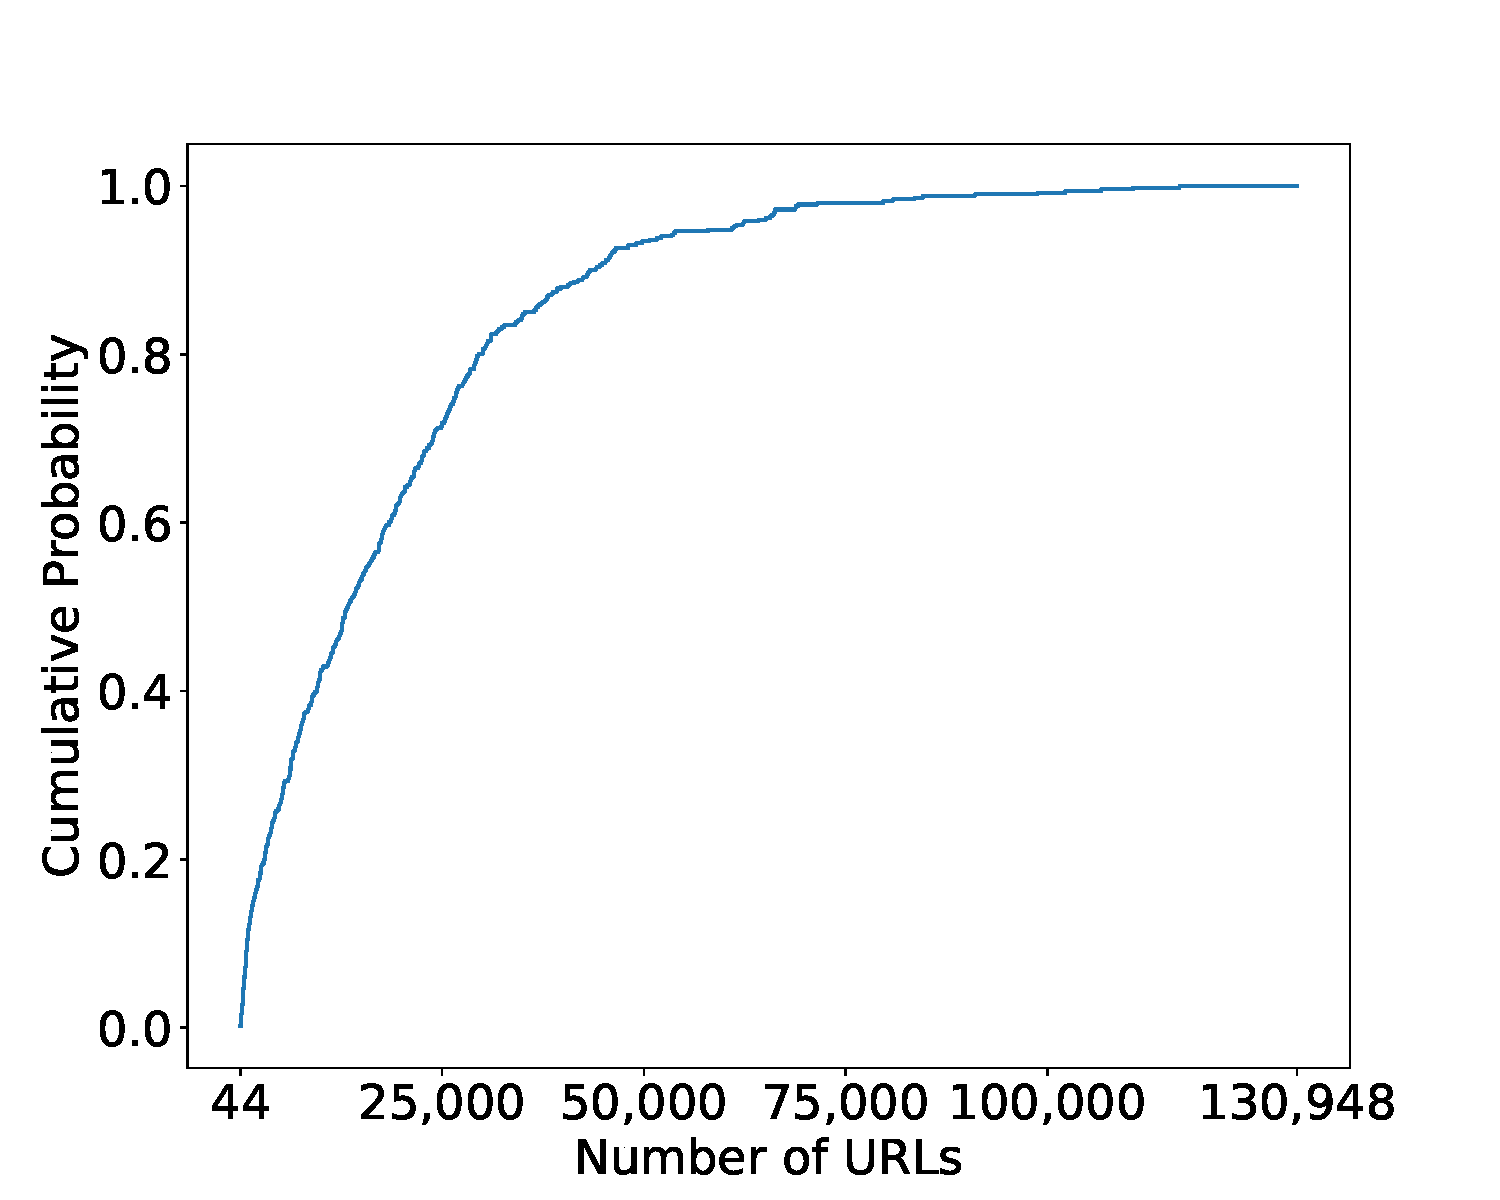
\includegraphics[scale=0.25]{summary_of_url-eps-converted-to.pdf}
    \caption{使用者瀏覽網頁數量之經驗分布函數}
    \label{fig:webcate_distribution}
    \end{center}
\end{figure}

\begin{table}[tbh]
    \centering 
    \caption{使用者瀏覽網頁數量之綜合統計} 
    \label{tab:url-stat-summary}
    \begin{tabular}{c|c|c|c|c|c} 
    \hline min & 1st Quartile & Median &Mean & 3rd Quartile & max \\
    \hline\hline $44$ & $4,239$ & $13,335$ & $19,103$ & $26,698$ & $130,992$ \\
    \hline
    \end{tabular} 
\end{table}

}
\subsection{資料集中使用者個人資訊之介紹}
{
全部具有網頁瀏覽紀錄的使用者之中共有 $508$ 位使用者具有較詳細的個人資訊(demographic information),個人資訊包含:性別、年齡以及感情狀態(單身、交往中、已婚以及其他),圖~\ref{fig:dataset_distribution} 以圓餅圖說明個人資訊之分布狀態。

\begin{figure}[h]
    \graphicspath{{fig/}}
    \begin{center}
    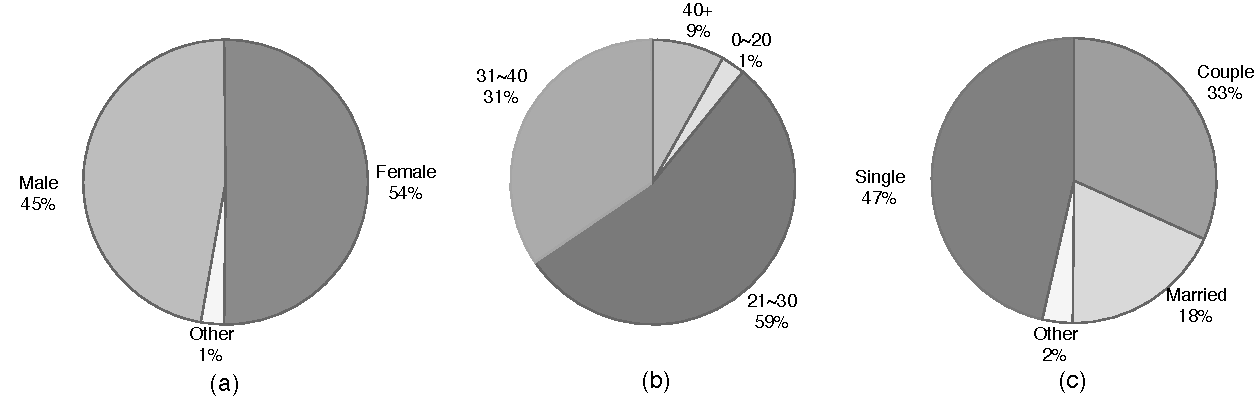
\includegraphics[scale=0.65]{fig/demo_pie.pdf}
    \caption{個人資訊分布狀態之圓餅圖,(a)性別(b)年齡(c)感情狀態}
    \label{fig:dataset_distribution}
    \end{center}
\end{figure}

}

\subsection{資料集中使用者大六性格特質之介紹}
{
全部具有網頁瀏覽紀錄之使用者中共有 $513$ 位使用者具大六性格特質測驗分數(big-six personality),其中大六性格特質包含:真誠性(Honesty-Humility)、情緒不穩定性(Neuroticism)、外向性(Extraversion)、親和性(Agreeableness)、盡責性(Conscientiousness)以及經驗開放性(Openness to Experience),各項分數分布狀態如圖~\ref{fig:pr_distribution}。大六性格特質為大五性格特質的延伸,大六性格特質增加了真誠性(Honesty-Humility)作為構成人的主要性格特徵,而大五性格特質在現代心理學中已經被認為是代表所有人格特質中的基本架構~\cite{o2002quantitative}。 \par

\begin{figure}[h]
    \graphicspath{{fig/}}
    \begin{center}
    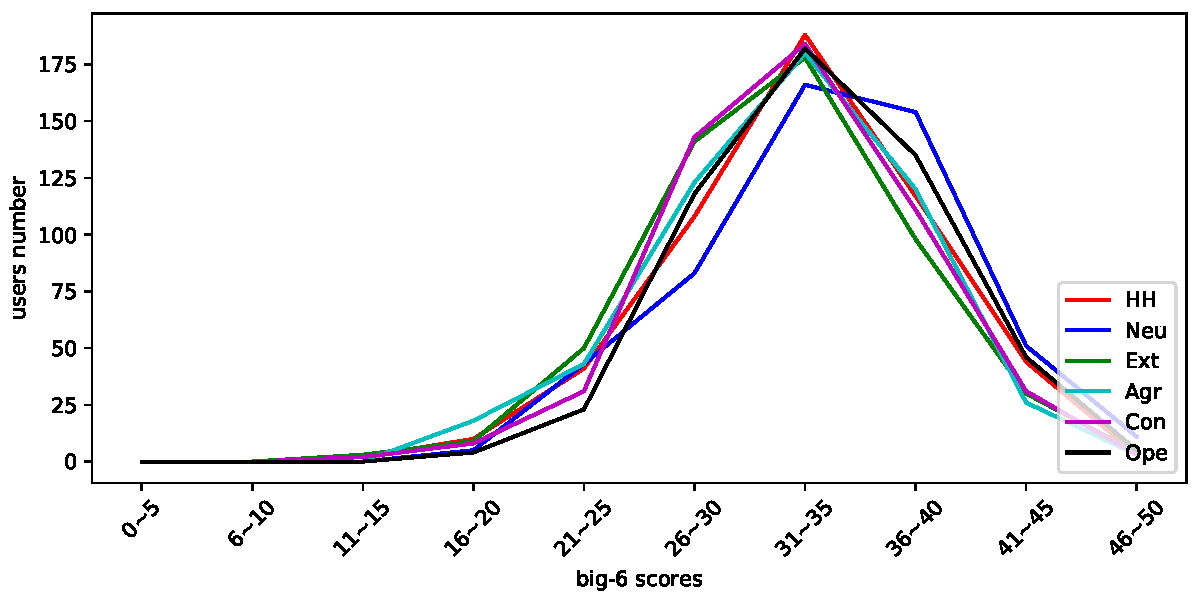
\includegraphics[scale=0.6]{fig/pr_dist.pdf}
    \caption{使用者之大六性格特質測驗分數分布狀態}
    \label{fig:pr_distribution}
    \end{center}
\end{figure}


使用者擁有三種資料集(使用者網頁瀏覽紀錄、使用者詳細個人資訊以及使用者之大六性格測驗分數)之間的人數集合關係可以透過圖~\ref{fig:dataset_distribution} 來了解,使用者具有網頁瀏覽紀錄人數為 $672$ 人,使用者具有詳細個人資訊之人數為 $508$ 人,使用者具有大六性格特質測驗分數為 $513$ 人,其中具有個人資訊之使用者皆具有大六性格特質測驗分數以及網頁瀏覽紀錄,而擁有大六性格特質測驗分數的使用者同時也擁有網頁瀏覽紀錄。

\begin{figure}[h]
    \graphicspath{{fig/}}
    \begin{center}
    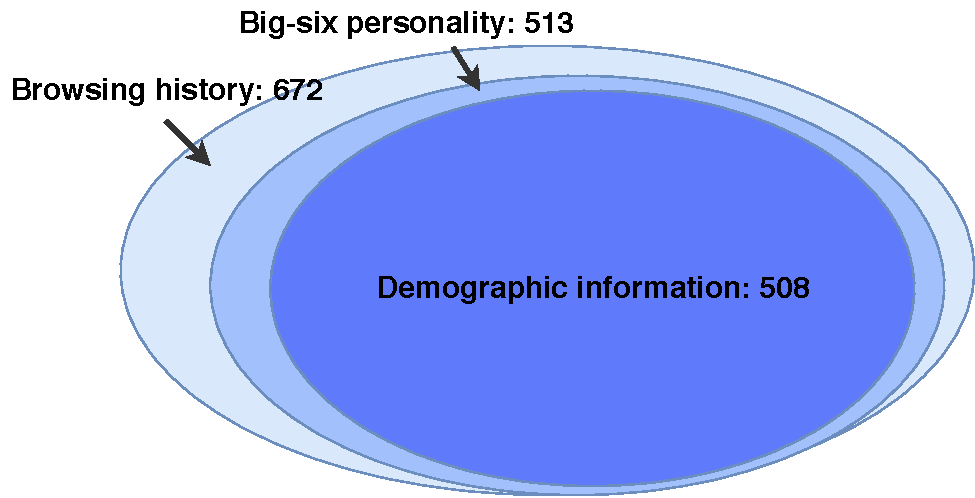
\includegraphics[scale=0.7]{fig/dataset_distribution.pdf}
    \caption{使用者中擁有三種資料集之間的人數集合關係}
    \label{fig:dataset_distribution}
    \end{center}
\end{figure}
}



\section{資料前處理之過程與想法}
{
原始資料集中分為三個部分,使用者之網頁瀏覽紀錄、使用者之個人資訊以及大六性格特質測驗分數,我將整體實驗架構訂為利用使用者之網頁瀏覽紀錄來預測使用者之個人資訊以及大六性格特質測驗分數。首先,我必須從使用者之網頁瀏覽紀錄找出特徵,起初我直接以使用者網頁瀏覽紀錄中的網址( URL)當作特徵,但是太多較為冷門的網頁只有極少部分的使用者瀏覽過,而熱門網頁所佔比例過高,例如:全部的使用者網頁瀏覽紀錄中最熱門之網頁為  facebook.com,佔全部網頁瀏覽紀錄的 $27.6\%$,圖~\ref{fig:url_popul} 為網頁瀏覽紀錄中的網址根據使用者瀏覽次數當作熱門程度之排名與使用者點擊次數之比較圖。基於此現象將造成特徵過於不平衡,所以我認為必須將特徵設定成網頁之種類較為合適。\par


因此資料前處理之第一步為將網頁瀏覽歷史紀錄中的網址(URL)透過網頁分類器進行分類\footnote{\url{http://www.fortiguard.com/webfilter}},網頁分類器能透過輸入網址後輸出對應的網頁類型,例如:輸入網址為 https://www.google.com/,則輸出之網頁類型為 “ Search Engines and Portals ”,以及輸入網址為 https://www.facebook.com/,則輸出之網頁類型為 “ Social Networking services ”。將所有使用者網頁瀏覽紀錄之網址進行分類後,總共包含88種網頁類型,進行統計後發現最熱門的網頁類型為 “ Social Networking services(SNS) ” 其次為 “ Search Engines and Portals ”,圖~\ref{fig:cate_pie} 為網頁類型佔所有瀏覽紀錄中之前五名之圓餅圖。\par

由於所有使用者網頁瀏覽歷史記錄的網址中最多瀏覽次數的網址前四名分別為 “ https://www.facebook.com/ ”、 “ https://www.google.com.tw/ ”、“ https:// mail.google.com/ ” 以及 “ https://www.youtube.com/ ”,分別佔全部的網頁瀏覽記錄中的 $27.6\%$、$11.8\%$、$6.6\%$ 以及 $6.4\%$,相對於其他網頁類型種類是相對高的,我最後再將這四種網址從網頁類別獨立出來當作 4 種獨立的網頁類型,因此網頁種類為 92 種。
}


\begin{figure}[h]
    \graphicspath{{fig/}}
    \begin{center}
    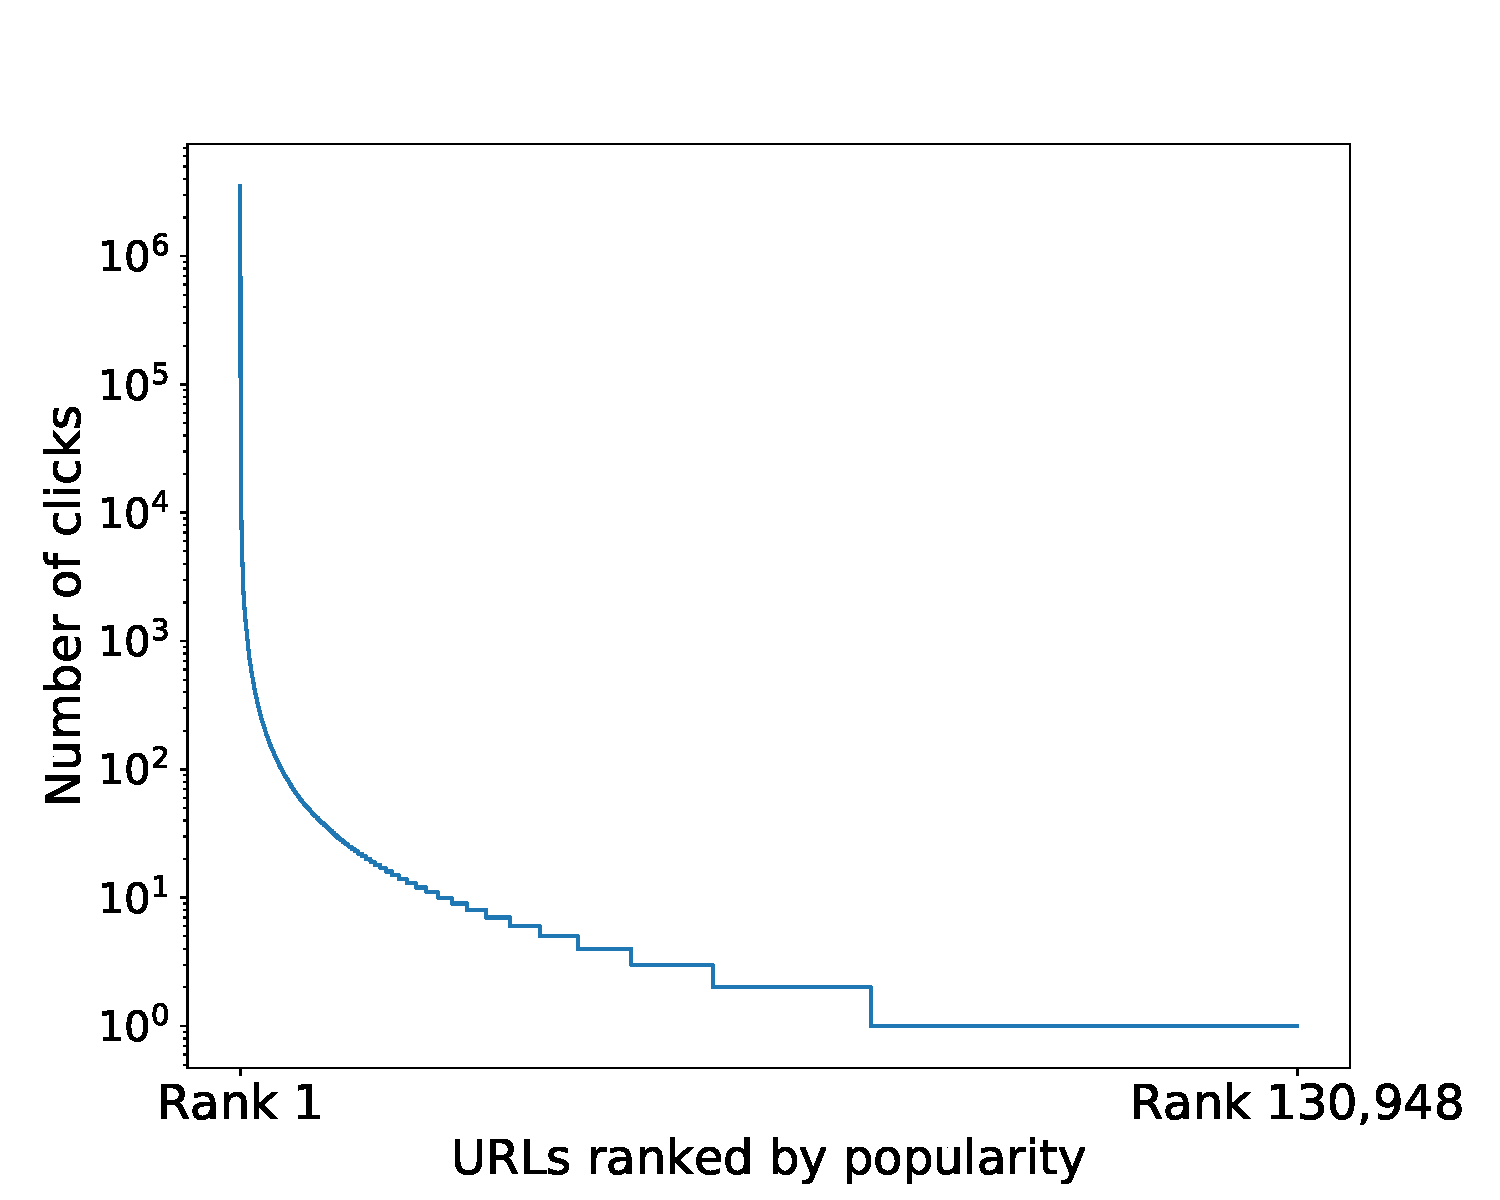
\includegraphics[scale=0.35]{fig/Proportion_of_url-eps-converted-to.pdf}
    \caption{使用者點擊次數與 URLs 熱門度排名之關係}
    \label{fig:url_popul}
    \end{center}
\end{figure}

\begin{figure}[h]
    \graphicspath{{fig/}}
    \begin{center}
    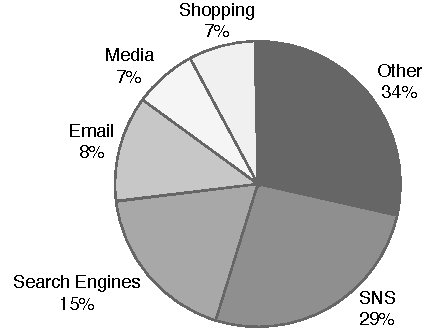
\includegraphics[scale=0.8]{fig/cate_pie.pdf}
    \caption{使用者網頁瀏覽紀錄之前五熱門類型種類比例}
    \label{fig:cate_pie}
    \end{center}
\end{figure}

\section{特徵選擇之原因以及分析}
{
呈 3.2 所說明將原始網頁瀏覽紀錄之網址轉化為網頁類型後,我將分為兩部分生成特徵,第一部分以使用者網頁瀏覽之類型作為依據,找出使用者之網頁瀏覽紀錄各類型網頁所佔之比例當作特徵,第二部分則是以使用者一天中在哪些時段瀏覽網頁之比例當作特徵。
}


\subsection{使用者於各類型網頁之瀏覽比例}
{
使用者之間的關聯性與瀏覽之網頁類型具有較高的關聯性,例如:年輕男性學生族群對於遊戲類型的網頁具有較高的瀏覽率,而銀行金融類型之網頁類型則對於年紀相對高的族群有較高的吸引力。因此以每一位使用者在各類型網頁的瀏覽比例當作特徵進行分析我認為是合適的選擇,而計算每一位使用者之在各類型網頁的瀏覽比例之算法為式(3.1),將使用者瀏覽過第 $i$ 種網頁類型之次數除以使用者之總瀏覽次數,作為使用者瀏覽第 $i$ 種網頁類型之比例,$cate_i$ $ratio$ 中 $i$ 為 $0\sim91$,分別代表 92 種不同的網頁類型。


    $$cate_i\mbox{ }ratio=\frac{\mbox{number of visits on the }cate_i\mbox{ websites}}{\mbox{total number of visits}} \eqno {(3.1)}$$

}

\section{使用者於一天中各時段之瀏覽頻率}
{
每一位使用者都有特定生活作息,我認為擁有類似生活作息的使用者之間可能擁有較高的關聯性,例如:大學生族群比較傾向晚睡,因此其在凌晨時段相對於其他使用者擁有較高的瀏覽比例。藉由使用者一天 24 個時段之中在各時段之瀏覽紀錄來統計每一位使用者在哪些時段瀏覽頻率較高,便能夠區分出各使用者族群。\par


其中定義使用者在同一天內擁有超過 30 筆瀏覽紀錄才能夠被認定當天有確切的瀏覽行為發生,並且在同一個時段內擁有超過 10 筆瀏覽紀錄才能夠被認定該時段確實有進行網頁瀏覽。而詳細的計算方式為式(3.2),使用者第 $i$ 個時段之網頁瀏覽頻率為使用者之網頁瀏覽紀錄中第 $i$ 個時段發生網頁瀏覽行為天數除以使用者有瀏覽行為天數總和,$timesession_i$ $ratio$中 $i$ 為 $0\sim23$,分別代表 0 時至 23 時之時段。

    $$timesession_i\mbox{ }ratio=\frac{\mbox{number of days have browsing behaviors in }timesession_i}{\mbox{number of days have browsing behaviors}} \eqno {(3.2)}$$
}


